As introduced in \cref{Introduction}, this thesis explores the generation of counterfactual explanations (CEs) in image-based autonomous driving scenarios using deep generative models and post-hoc interpretability techniques. The corresponding implementations are detailed in \cref{Methodology}.

This chapter presents the evaluation strategy and experimental findings, structured according to the central research questions (RQs). For each RQ, the evaluation criteria are outlined and later expanded in dedicated result sections.

\textbf{RQ1:} \textit{How can deep generative models be implemented to effectively encode and reconstruct images of high-dimensional driving scenes for interpretable and compact representation learning in autonomous driving systems?}

    \subsubsection*{Evaluation} 
    The VAE is evaluated on two primary fronts: (i) the fidelity of reconstructed images, and (ii) the semantic usefulness of the latent representations for downstream classification. To this end, multiple classifiers—including MLP, SVM, KNN, Logistic Regression, and Random Forest—are trained on the latent vectors extracted by the encoder. Classification performance is assessed for both binary (GO vs. STOP) and multi-class (GO, STOP, LEFT, RIGHT) tasks. Evaluation metrics include reconstruction loss, pixel accuracy, PSNR, classification accuracy, precision, recall, and F1-score.
    
\textbf{RQ2:} \textit{How can loss function modifications in Variational Autoencoders (VAEs) optimize image reconstruction quality in autonomous driving tasks?} 

    \subsubsection*{Evaluation} 
    Compare the image quality Structural Similarity Index (SSIM) and Peak Signal-to-Noise Ratio (PSNR) and classification metrics (accuracy, F1) between a standard VAE and one using modified loss functions. This will include both quantitative analysis and qualitative visualizations of reconstructed images.
    
\textbf{RQ3:} \textit{How do different masking techniques impact the effectiveness and efficiency of counterfactual explanation generation, in terms of coverage, computational cost, method overlap, and failure rate? (See \cref{Methodology} for details on the techniques investigated.)}

    \subsubsection*{Evaluation}
    To assess each method, the following criteria are measured during CE generation:
    \begin{itemize}
        \item \textbf{Coverage:} Proportion of total inputs for which valid counterfactual explanations are successfully generated.
        \item \textbf{Computational Cost:} Average time taken per sample for each method.
        \item \textbf{Failure Rate:} Percentage of inputs for which no counterfactual explanations was found.
        \item \textbf{Method Overlap:} Instances where multiple masking techniques generate the same counterfactual explanations.
        \item \textbf{Visual Quality:} SSIM, PSNR, UQI, and VIFP metrics between original and reconstructed images.
    \end{itemize}

    All masking methods are applied to the same dataset split, using identical model checkpoints for the VAE and classifier. This ensures fair and consistent comparisons across metrics.
    
\textbf{RQ4:} \textit{ Which counterfactual explanation method is preferred by users when selecting among generated explanations of the same original image? What factors (interpretability, plausibility, and visual coherence) influence user preference? (See \cref{Methodology} for details on the methods compared.)}

    \subsubsection*{Evaluation}
    Evaluation is based on aggregated user responses:
    
    \begin{itemize}
        \item \textbf{Preference Distribution:} Percentage of total selections made per CE method.
        \item \textbf{Attribute Ratings:} Average scores for interpretability, plausibility, and coherence across methods.
        \item \textbf{Qualitative Feedback:} Comments collected through optional text fields to gain insights into user reasoning.
        \item \textbf{Inter-method Comparison:} Correlation between user ratings and quantitative CE quality metrics (e.g. SSIM, PSNR).
    \end{itemize}

    This dual analysis enables the identification of methods that are not only algorithmically effective but also intuitively meaningful to end users critical for real-world deployment of interpretable AI in autonomous systems.
    


Each of the following sections restates the respective RQ, evaluates the implemented methods against that question, and presents results along with a discussion of key findings.


\subsection{Evaluation of Variational Autoencoder (VAE)} \label{subsec:vae_evaluation}

The Variational Autoencoder (VAE) forms the backbone of this thesis. It serves dual purposes: (i) as a deep generative model that enables the reconstruction and manipulation of high-dimensional driving scene images, and (ii) as a representation learning tool to generate low-dimensional, semantically meaningful latent vectors suitable for downstream driving action classification. The quality of both image reconstruction and latent encoding is crucial for the success of counterfactual generation. Therefore, evaluating the VAE both quantitatively and qualitatively is a vital first step.

To ensure robustness, various architectural configurations and hyperparameter settings were explored, including latent dimensionality, convolutional depth, and KL divergence annealing schedules. One major focus was the choice of reconstruction loss function, which has a significant effect on the quality of output and the stability of training. Two variants were trained. One using traditional Mean Squared Error (MSE) and the other using Log-Cosh, a smoother, outlier-robust alternative motivated by prior work by Chen et al.,~\cite{chen2019log}. This section presents the training dynamics, comparative results between the two losses, and the final analysis of latent space quality.

\subsubsection{Training Performance and Loss Analysis} \label{subsubsec:vae_training_loss}

Two VAE variants were trained for 200 epochs each, differing only in their reconstruction loss: Mean Squared Error (MSE) and Log-Cosh. Throughout training, we monitored several key metrics:

\begin{itemize}
    \item \textbf{Total Loss:} Sum of reconstruction and KL divergence losses.
    \item \textbf{Reconstruction Loss:} Measures pixel-wise reconstruction error.
    \item \textbf{KL Divergence:} Reflects the alignment of the latent space distribution with a unit Gaussian prior.
    \item \textbf{Validation Pixel Accuracy:} Measures how accurately the reconstructed image matches the original at pixel level.
    \item \textbf{PSNR (Peak Signal-to-Noise Ratio):} Evaluates perceptual reconstruction quality.
\end{itemize}

\textbf{Log-Cosh Variant (Figures \ref{fig:logcosh_kl_loss} to \ref{fig:logcosh_psnr})}

\begin{itemize}
    \item \textbf{KL Divergence:} As shown in Figure~\ref{fig:logcosh_kl_loss}, KL loss rapidly decreased in the early epochs and gradually stabilized, indicating that the annealing schedule successfully encouraged disentangled latent features.
    \item \textbf{Reconstruction \& Total Loss:} Both training and validation losses (Figures~\ref{fig:logcosh_recon_loss} and \ref{fig:logcosh_total_loss}) show a smooth, monotonic decrease, suggesting stable convergence.
    \item \textbf{Pixel Accuracy \& PSNR:} Validation pixel accuracy steadily increased, reaching 0.97 (Figure~\ref{fig:logcosh_val_acc}), while PSNR improved consistently to 31.4 dB (Figure~\ref{fig:logcosh_psnr}).
\end{itemize}

A qualitative comparison of the reconstructed image at epoch 200 (Figure~\ref{fig:logcosh_epoch200}) shows that the VAE preserves semantic structure and texture remarkably well.

\begin{figure}[htbp]
    \centering
    \begin{subfigure}[b]{0.45\textwidth}
        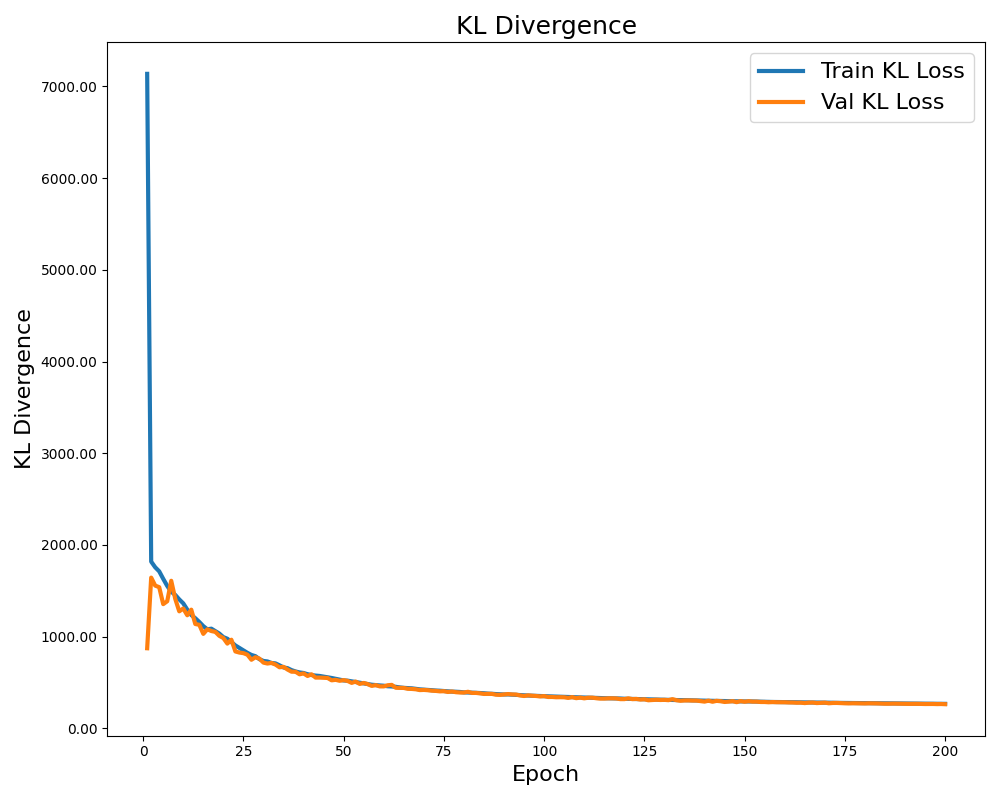
\includegraphics[width=\textwidth]{img/vae_results/200_epochs_128_ls_logcosh/logcosh_kl_loss.png}
        \caption{KL divergence over epochs for VAE trained with Log-Cosh loss.}
        \label{fig:logcosh_kl_loss}
    \end{subfigure}
    \hfill
    \begin{subfigure}[b]{0.45\textwidth}
        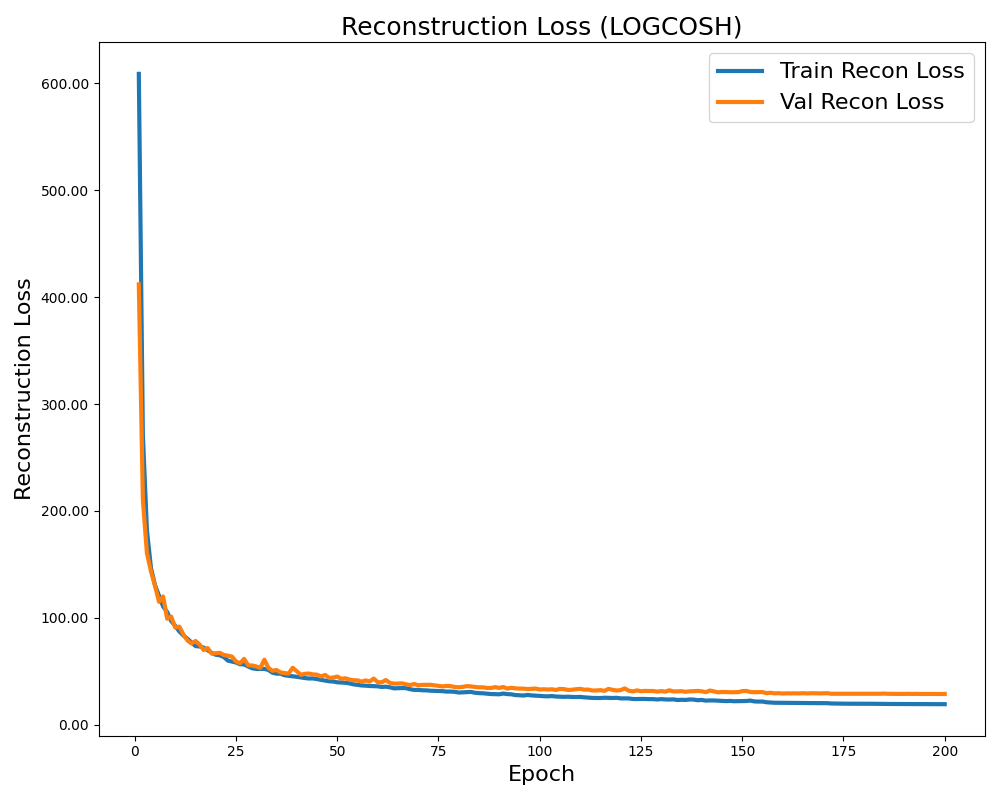
\includegraphics[width=\textwidth]{img/vae_results/200_epochs_128_ls_logcosh/logcosh_recon_loss.png}
        \caption{Reconstruction loss over epochs (Log-Cosh).}
        \label{fig:logcosh_recon_loss}
    \end{subfigure}
    
    \begin{subfigure}[b]{0.45\textwidth}
        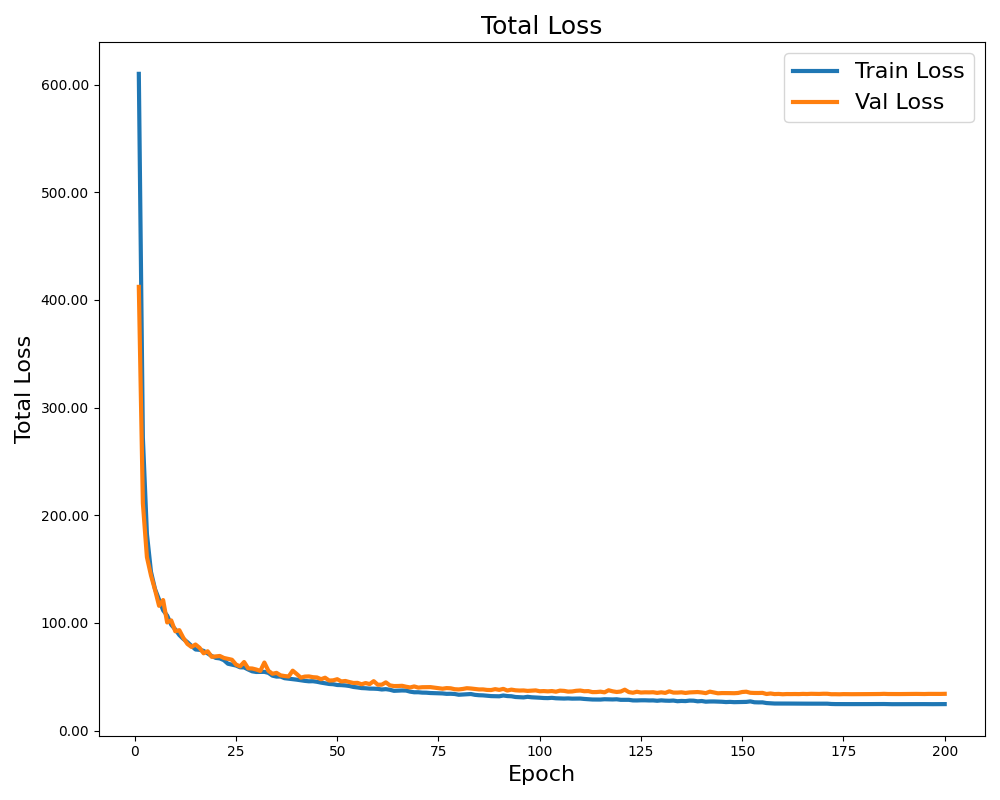
\includegraphics[width=\textwidth]{img/vae_results/200_epochs_128_ls_logcosh/logcosh_total_loss.png}
        \caption{Total loss over epochs (Log-Cosh).}
        \label{fig:logcosh_total_loss}
    \end{subfigure}
    \hfill
    \begin{subfigure}[b]{0.45\textwidth}
        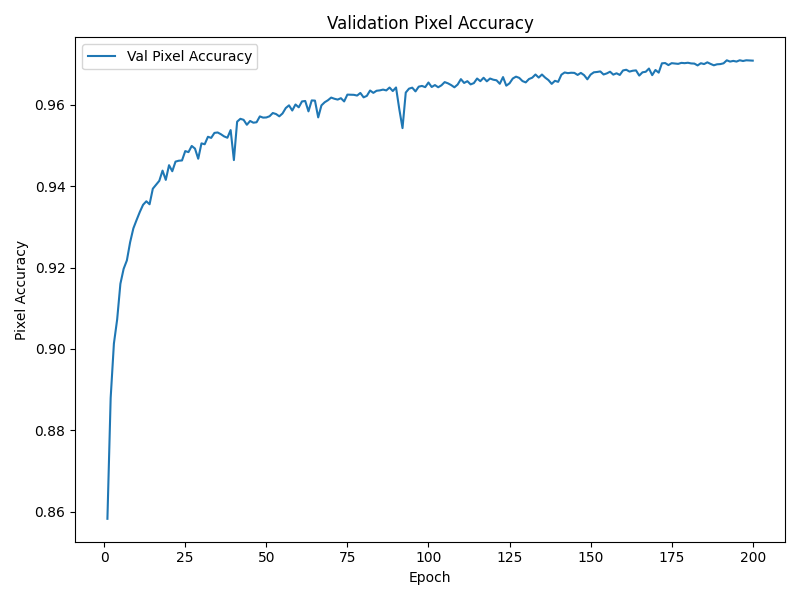
\includegraphics[width=\textwidth]{img/vae_results/200_epochs_128_ls_logcosh/logcosh_val_accuracy.png}
        \caption{Validation pixel accuracy across epochs (Log-Cosh).}
        \label{fig:logcosh_val_acc}
    \end{subfigure}
    
    \begin{subfigure}[b]{0.45\textwidth}
        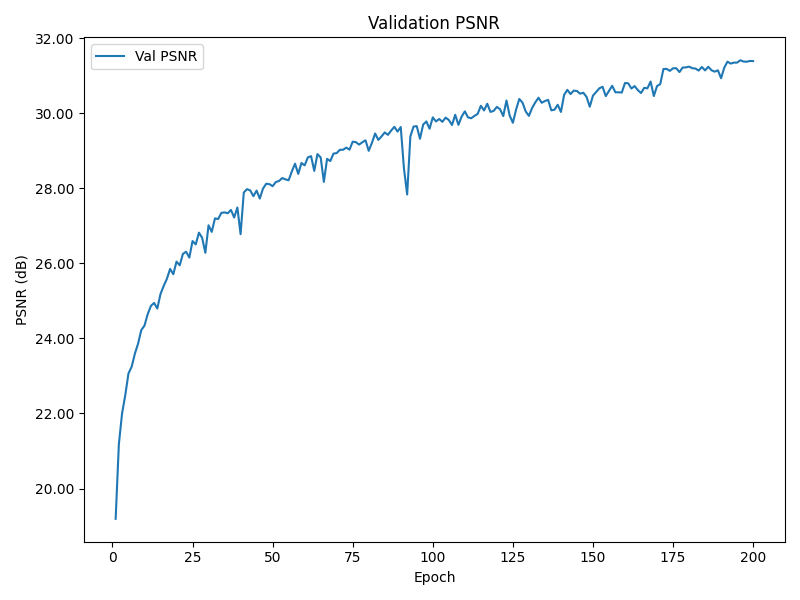
\includegraphics[width=\textwidth]{img/vae_results/200_epochs_128_ls_logcosh/logcosh_val_psnr.png}
        \caption{Validation PSNR trajectory for Log-Cosh model.}
        \label{fig:logcosh_psnr}
    \end{subfigure}
    \hfill
    \begin{subfigure}[b]{0.45\textwidth}
        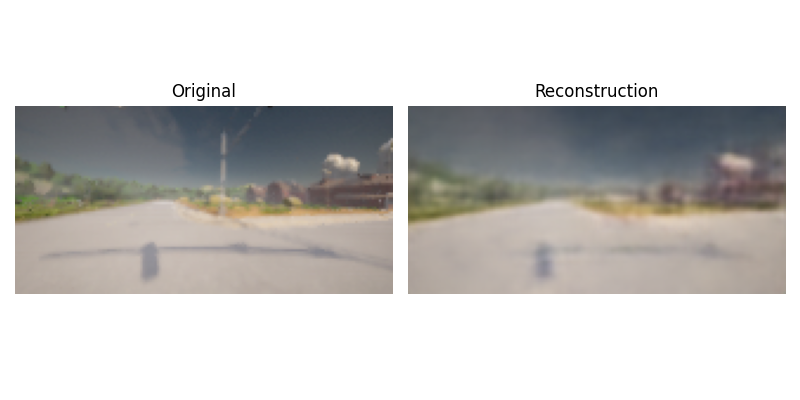
\includegraphics[width=\textwidth]{img/vae_results/200_epochs_128_ls_logcosh/reconstructions/epoch_200.png}
        \caption{Original vs. Reconstructed image at epoch 200 (Log-Cosh).}
        \label{fig:logcosh_epoch200}
    \end{subfigure}
    
    \caption{Training Performance and Loss Analysis for Log-Cosh Variant: Detailed analysis of the VAE's performance using the Log-Cosh loss function, highlighting key metrics and qualitative results.}
    \label{fig:logcosh_analysis}
\end{figure}




\subsubsection{Training Comparison with MSE Loss} \label{subsubsec:vae_mse_loss}

The training curves for the MSE-based VAE show similar convergence trends but at a consistently higher loss level across all metrics:

\begin{itemize}
    \item \textbf{Total and Reconstruction Loss:} Figures~\ref{fig:mse_total_loss} and \ref{fig:mse_recon_loss} indicate slower and less stable convergence compared to Log-Cosh.
    \item \textbf{Pixel Accuracy \& PSNR:} Slightly lower final accuracy (~0.969) and PSNR (30.99 dB), as seen in Figures~\ref{fig:mse_val_acc} and \ref{fig:mse_val_psnr}.
\end{itemize}

Qualitative Comparison: Figure~\ref{fig:mse_epoch200} shows noticeable blur and loss of fine structure in the reconstructions compared to Log-Cosh.

\begin{figure}[htbp]
    \centering
    \begin{subfigure}[b]{0.45\textwidth}
        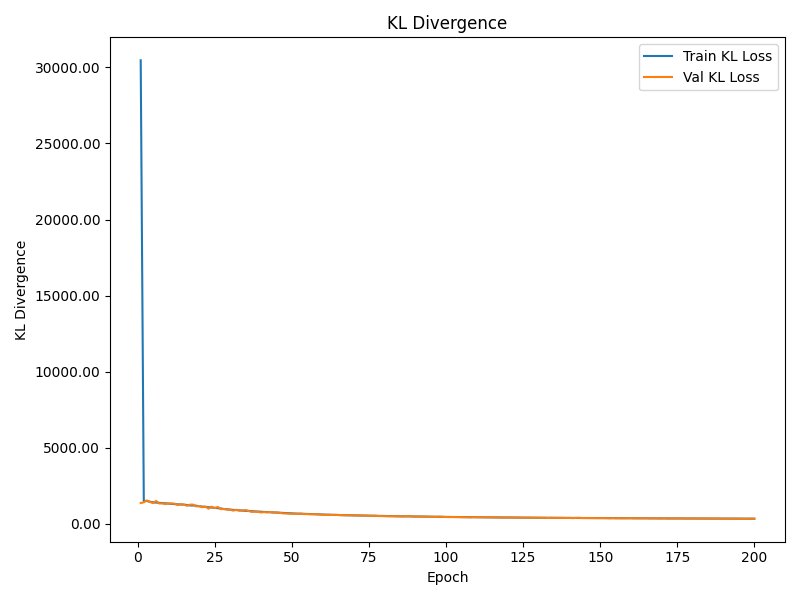
\includegraphics[width=\textwidth]{img/vae_results/200_epochs_128_ls_mse/mse_kl_loss.png}
        \caption{KL divergence over epochs for VAE trained with MSE loss.}
        \label{fig:mse_kl_loss}
    \end{subfigure}
    \hfill
    \begin{subfigure}[b]{0.45\textwidth}
        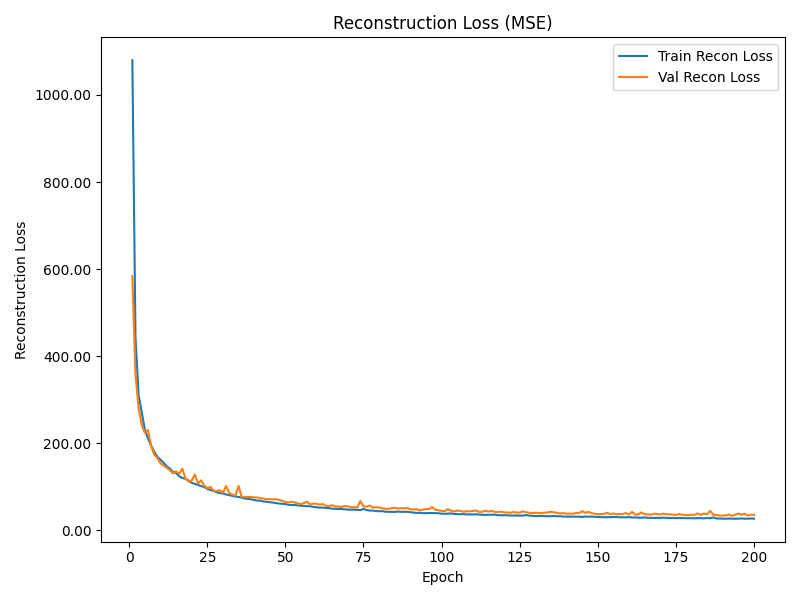
\includegraphics[width=\textwidth]{img/vae_results/200_epochs_128_ls_mse/mse_recon_loss.png}
        \caption{Reconstruction loss over epochs (MSE).}
        \label{fig:mse_recon_loss}
    \end{subfigure}
    
    \begin{subfigure}[b]{0.45\textwidth}
        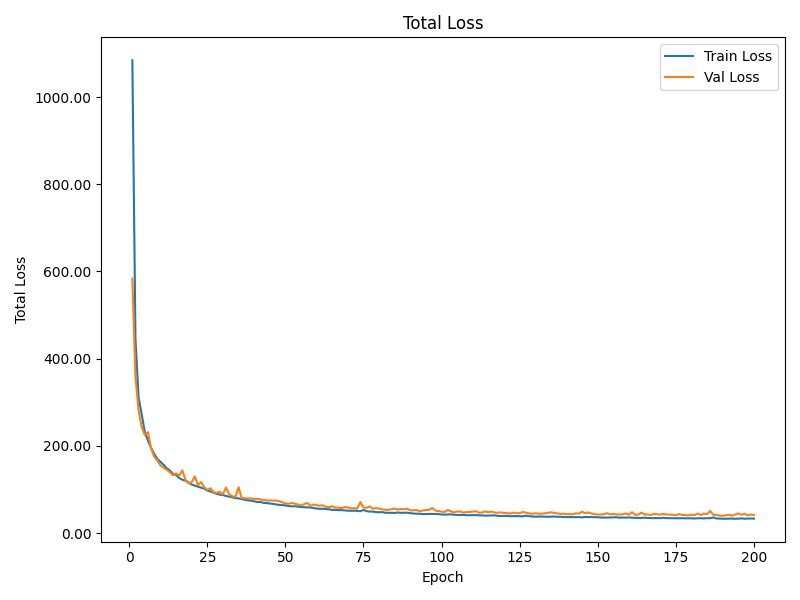
\includegraphics[width=\textwidth]{img/vae_results/200_epochs_128_ls_mse/mse_total_loss.png}
        \caption{Total loss over epochs (MSE).}
        \label{fig:mse_total_loss}
    \end{subfigure}
    \hfill
    \begin{subfigure}[b]{0.45\textwidth}
        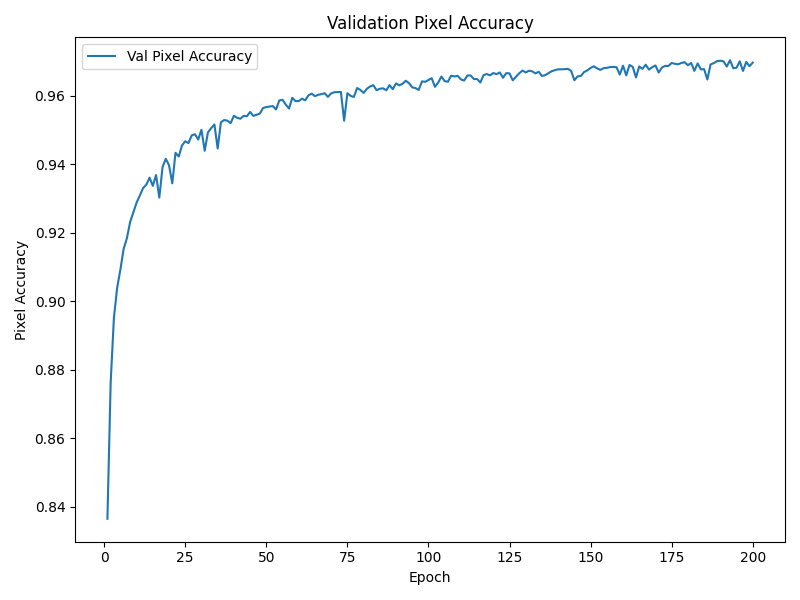
\includegraphics[width=\textwidth]{img/vae_results/200_epochs_128_ls_mse/mse_val_accuracy.png}
        \caption{Validation pixel accuracy across epochs (MSE).}
        \label{fig:mse_val_acc}
    \end{subfigure}
    
    \begin{subfigure}[b]{0.45\textwidth}
        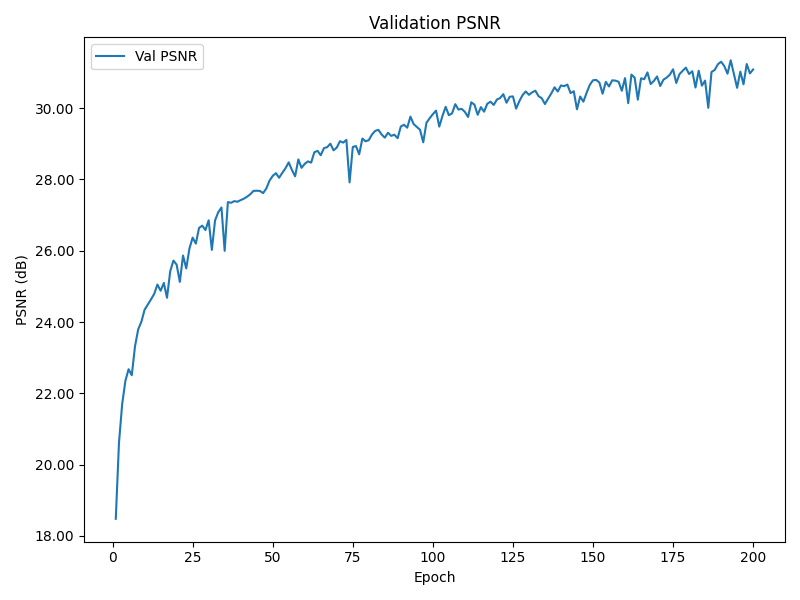
\includegraphics[width=\textwidth]{img/vae_results/200_epochs_128_ls_mse/mse_val_psnr.png}
        \caption{Validation PSNR trajectory for MSE model.}
        \label{fig:mse_val_psnr}
    \end{subfigure}
    \hfill
    \begin{subfigure}[b]{0.45\textwidth}
        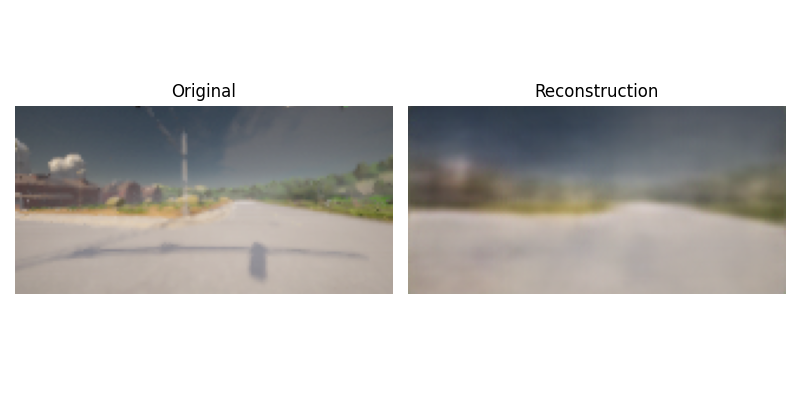
\includegraphics[width=\textwidth]{img/vae_results/200_epochs_128_ls_mse/reconstructions/epoch_200.png}
        \caption{Original vs. Reconstructed image at epoch 200 (MSE).}
        \label{fig:mse_epoch200}
    \end{subfigure}
    
    \caption{Training Performance and Loss Analysis for MSE Variant: A comparison of the VAE's performance using MSE loss, highlighting differences in convergence and reconstruction quality compared to Log-Cosh.}
    \label{fig:mse_analysis}
\end{figure}










\subsubsection{Quantitative Comparison of Loss Functions} \label{subsubsec:vae_quant_comparison}
To assess the performance of the Variational Autoencoder (VAE), both the Log-Cosh and Mean Squared Error (MSE) loss functions were evaluated across several metrics, namely Total Loss, Reconstruction Loss, KL Divergence, Validation Pixel Accuracy, Peak Signal-to-Noise Ratio (PSNR). 

Table~\ref{tab:loss_comparison} presents average values over the final 5 epochs for both variants:

\begin{table}[htbp]
    \centering
    \begin{tabular}{lcc}
        \toprule
        \textbf{Metric} & \textbf{Log-Cosh (Avg)} & \textbf{MSE (Avg)} \\
        \midrule
        Validation Total Loss & 21.82 & 42.35 \\
        Validation Reconstruction Loss & 16.49 & 35.84 \\
        Validation KL Divergence & 268.72 & 327.90 \\
        Validation Pixel Accuracy & 0.971 & 0.969 \\
        Validation PSNR (dB) & 31.39 & 30.99 \\
        \bottomrule
    \end{tabular}
    \caption{Comparison of validation metrics for VAE variants (Final 5 Epoch Average)}
    \label{tab:loss_comparison}
\end{table}

Additionally, Figures~\ref{fig:val_loss_comparison} and \ref{fig:val_psnr_comparison} provide a side-by-side comparison of Validation Loss and PSNR over all epochs.




\begin{figure}[htbp]
    \centering
    \begin{subfigure}[b]{0.49\textwidth}
        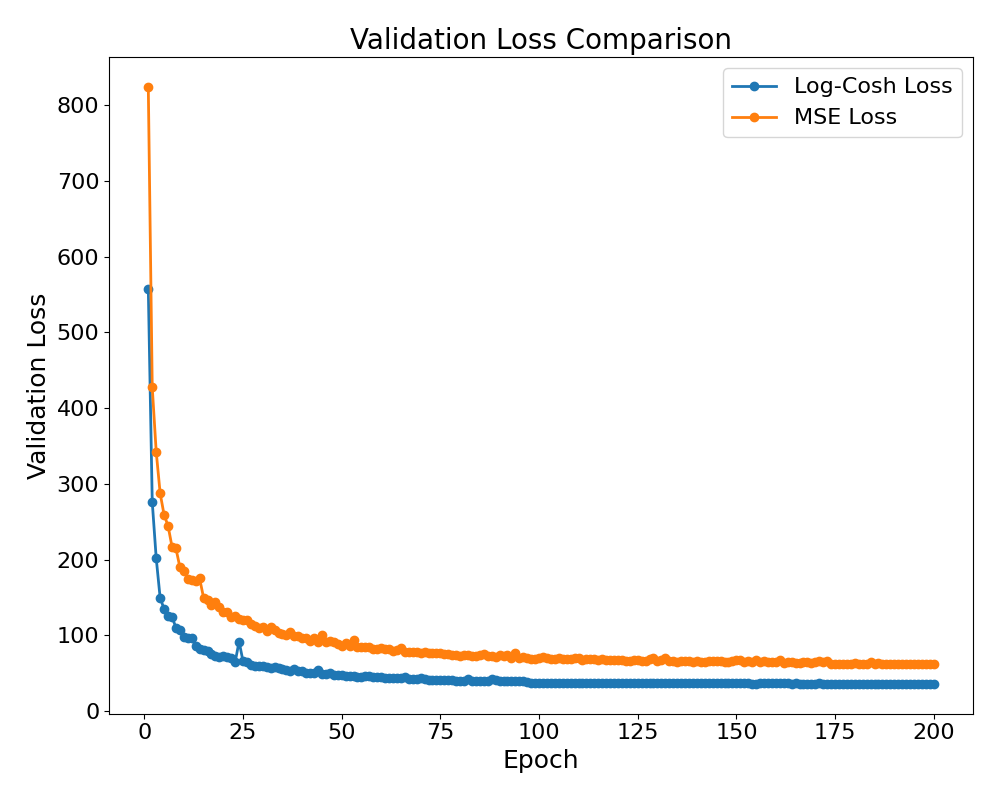
\includegraphics[width=\textwidth]{img/vae_results/val_loss_comparison.png}
        \caption{Validation Loss Comparison: Log-Cosh vs. MSE over all epochs.}
        \label{fig:val_loss_comparison}
    \end{subfigure}
    \hfill
    \begin{subfigure}[b]{0.49\textwidth}
        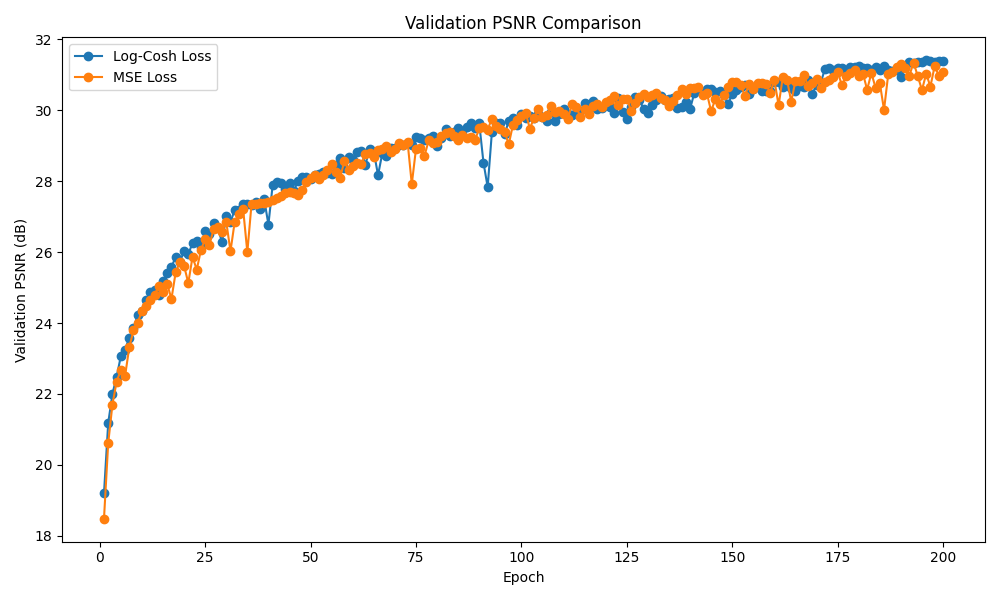
\includegraphics[width=\textwidth]{img/vae_results/val_psnr_comparison.png}
        \caption{Validation PSNR Comparison: Log-Cosh vs. MSE over all epochs.}
        \label{fig:val_psnr_comparison}
    \end{subfigure}
    
    \caption{Quantitative Comparison of Loss Functions: Validation Loss and PSNR for Log-Cosh and MSE variants.}
    \label{fig:quant_comparison}
\end{figure}


From these results:

\begin{itemize}
    \item The Log-Cosh loss outperformed MSE in terms of both total and reconstruction loss, indicating smoother training and better pixel-wise fidelity.
    \item A higher PSNR suggests improved perceptual quality in reconstructions when using Log-Cosh.
    \item KL Divergence was slightly lower for Log-Cosh, indicating a better balance between compression and regularization.
    \item These results affirm the hypothesis that the Log-Cosh loss leads to more visually realistic reconstructions, thus answering RQ2.
\end{itemize}



\subsubsection{Visual Comparison of Reconstructions} \label{subsubsec:vae_visual_recon}
Representative input images and corresponding reconstructions from both models at epoch 200 were visually compared.

Log-Cosh Reconstructions (Figure~\ref{fig:logcosh_epoch200}) retain road boundaries, tree textures, and lighting gradients with greater smoothness and fewer artifacts.

MSE Reconstructions (Figure~\ref{fig:mse_epoch200}) exhibit noise in edge regions and less coherent texture patterns and lost many important details like traffic light pole, road boundary and many more.

These qualitative results further confirms that adopting the Log-Cosh loss, as motivated by Chen et al.~\cite{chen2019log}, substantially improves VAE performance thereby answering RQ2 (How can loss function modifications in Variational Autoencoders (VAEs) optimize image reconstruction quality in autonomous driving tasks?).







\subsection{Neural Classifier on Latent Features (4-Class)}

To evaluate the performance of the neural network classifier trained on VAE extracted latent features, both quantitative metrics and qualitative visualizations were analyzed.

The model was trained for 20 epochs in the 4-class dataset (\texttt{STOP}, \texttt{GO}, \texttt{RIGHT}, \texttt{LEFT}) using the training set of 13,308 samples and evaluated on a held-out test set of 3,284 samples. The training progression is shown in Figure~\ref{fig:loss_accuracy_plot}.

\begin{figure}[h]
    \centering
    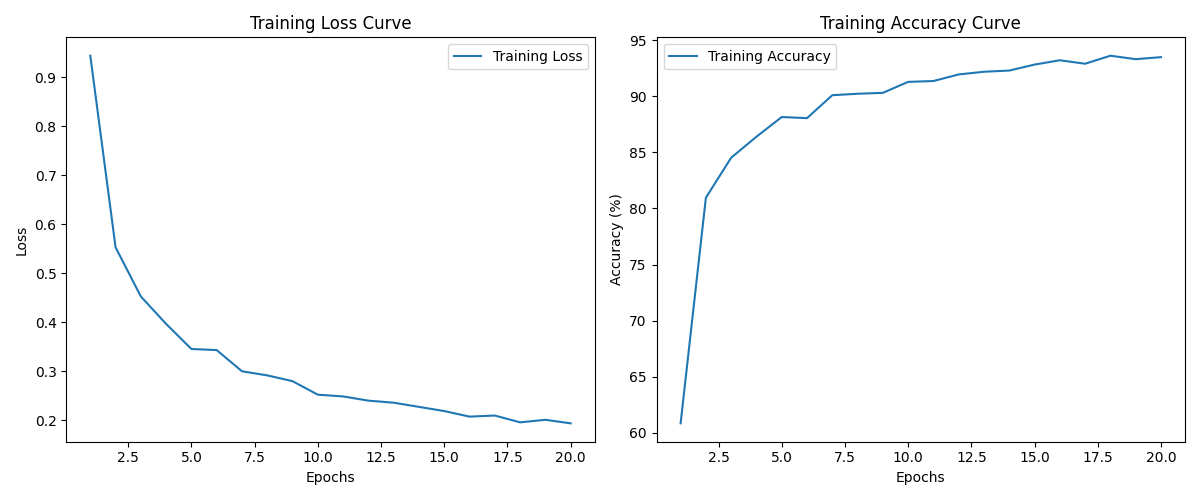
\includegraphics[width=\textwidth]{img/classifier/training_loss_accuracy_4_classes.png}
    \caption{Training loss and accuracy curves for the neural classifier.}
    \label{fig:loss_accuracy_plot}
\end{figure}

The training curves indicate a steady decrease in loss and improvement in accuracy, reaching a final training accuracy of approximately 89.4\%. This suggests the model learned meaningful patterns from the latent features without overfitting.

\subsubsection*{Classification Report}

Table~\ref{tab:classification_report} summarizes the classifier's performance on each class using precision, recall, and F1-score:

\begin{table}[h]
\centering
\begin{tabular}{lcccc}
\toprule
\textbf{Class} & \textbf{Precision} & \textbf{Recall} & \textbf{F1-score} & \textbf{Support} \\
\midrule
STOP  & 0.91 & 0.99 & 0.95 & 821 \\
GO    & 0.81 & 0.84 & 0.83 & 821 \\
RIGHT & 0.93 & 0.86 & 0.89 & 821 \\
LEFT  & 0.93 & 0.89 & 0.91 & 821 \\
\midrule
\textbf{Accuracy} & \multicolumn{4}{c}{0.89 (3284 samples)} \\
\textbf{Macro avg} & 0.90 & 0.89 & 0.89 & -- \\
\textbf{Weighted avg} & 0.90 & 0.89 & 0.89 & -- \\
\bottomrule
\end{tabular}
\caption{Classification report for the neural classifier (4-class).}
\label{tab:classification_report}
\end{table}

\subsubsection*{Confusion Matrix}

The confusion matrix in Figure~\ref{fig:conf_matrix} provides further insight into class-wise misclassifications:

\begin{figure}[h]
    \centering
    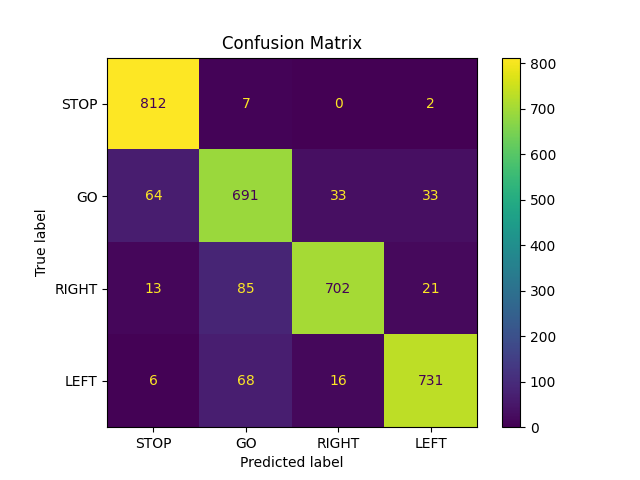
\includegraphics[width=0.6\textwidth]{img/classifier/confusion_matrix_4_classes.png}
    \caption{Confusion matrix for the neural classifier on the 4-class test set.}
    \label{fig:conf_matrix}
\end{figure}

\textbf{Observations:}
\begin{itemize}
    \item \textbf{STOP:} Most accurately classified class with a recall of 0.99.
    \item \textbf{GO:} Relatively weaker precision and recall; misclassified as \texttt{RIGHT} or \texttt{LEFT} in 8\% of cases.
    \item \textbf{RIGHT:} High precision, but some overlap with \texttt{GO} (85 misclassifications).
    \item \textbf{LEFT:} Very strong performance overall, with some confusion with \texttt{GO}.
\end{itemize}

These results confirm that the classifier is highly capable of distinguishing most driving actions using VAE latent features, though the \texttt{GO} class remains the most ambiguous.




\subsection{Comparison with Traditional Classifiers}

To contextualize the performance of the neural network classifier, a suite of traditional machine learning models were trained and evaluated on the same latent feature representations extracted from the VAE. These models include Logistic Regression, K-Nearest Neighbors (KNN), Support Vector Machine (SVM), and Random Forest. Each model was trained on the 128-dimensional latent vectors and tested on the same 4-class dataset.

Table~\ref{tab:classifier_comparison} presents a side-by-side comparison of accuracy and F1-scores across all classifiers:

\begin{table}[h]
\centering
\small 
\begin{tabular}{p{2.5cm}ccp{3.5cm}}
\toprule
\textbf{Classifier} & \textbf{Accuracy} & \textbf{Macro F1} & \textbf{Notes} \\
\midrule
Logistic Regression & 80\% & 0.80 & Baseline linear classifier; struggled with \texttt{GO} \\[2pt]
KNN & 88\% & 0.88 & High recall for \texttt{STOP}, sensitive to latent proximity \\[2pt]
SVM & 89\% & 0.89 & Excellent class separability; especially for \texttt{LEFT} and \texttt{STOP} \\[2pt]
Random Forest & 88\% & 0.88 & Robust performance; most errors in \texttt{GO} class \\[2pt]
Neural Network & \textbf{89\%} & \textbf{0.89} & Best overall F1 balance; handles non-linear separations \\
\bottomrule
\end{tabular}
\caption{Performance comparison of classifiers trained on VAE latent features (4-class).}
\label{tab:classifier_comparison}
\end{table}

\textbf{Key Observations:}
\begin{itemize}
    \item The neural classifier and SVM achieved the highest overall accuracy and macro F1-score (both 0.89), indicating strong class separation in the latent space.
    \item Logistic Regression performed the weakest, highlighting the limitation of linear decision boundaries in this latent representation.
    \item KNN and Random Forest both achieved strong results, particularly for the \texttt{STOP} class, but showed more confusion on the \texttt{GO} class.
    \item Across all models, the \texttt{GO} class consistently had the lowest precision and recall, suggesting overlapping representations in the latent space that merit further exploration.
\end{itemize}

These results confirm the value of the VAE latent space as a compact and expressive representation, allowing both deep and traditional classifiers to achieve competitive performance on complex multi-class driving data.
r. 













\section{Evaluation of Masking Methods} \label{sec:evaluation}
To address \textbf{RQ3} (see Section~\ref{sec:research_question}), we performed a comprehensive evaluation of all implemented masking techniques across multiple dimensions: counterfactual coverage, computational efficiency, method overlap, and robustness. A custom Python script was developed to automate the analysis by aggregating and comparing the results from each method's output CSV files.

The script computes the total number of counterfactual explanations (CEs) found per method, their distribution across class labels, and the overall time taken. It also generates:

\begin{itemize}
    \item \textbf{Venn diagrams} illustrating overlaps in images where different methods found CEs,
    \item \textbf{Bar charts} summarizing the count of successful explanations,
    \item \textbf{Comparison tables} detailing which images were explained by which method,
    \item \textbf{Overlap summaries} categorizing all images based on individual or shared method success,
    \item \textbf{Sanity checks} verifying consistency and correctness in prediction changes,
    \item \textbf{Validity checks} ensuring the reconstructed images are plausible (via SSIM, PSNR, etc.).
\end{itemize}

These results are saved as CSV and high-resolution plots and are discussed in detail in Section~\ref{sec:results_and_discussion}.




\section{Overview of the Evaluation Strategy}
Counterfactuals were evaluated using both AI-based metrics and human evaluation.

\section{AI-Based Quantitative Evaluation}

\subsection{Evaluating the VAE Reconstruction Performance}
traditional loss like MSE loss vs logcosh loss comparison.
The SSIM and PSNR scores were computed to measure the quality of image reconstructions.
A visualization of reconstructed vs. original images was analyzed.

To evaluate the quality of the counterfactual explanations generated by our three methods: 
\textbf{Grid-Based Masking, LIME on Images, LIME on Latent Features}, we collected user ratings based on three criteria: 
\textbf{Interpretability, Plausibility, Visual Coherence}. Users rated each counterfactual on a scale of 1 (poor) to 5 (excellent). 
The collected data were stored in a CSV file, and we computed the mean ratings for each method and criterion.


\subsection{Counterfactual Success Rate (CSR) Across Different Masking Methods}
CSR measures how often a counterfactual successfully flips the classifier’s decision.
Comparison of CSR across different masking methods:
LIME on Latent Features: X%
Grid-Based Masking: Y%
Object Detection-Based Masking: Z%
LIME on Images: W%


\subsection{Structural and Visual Quality of Counterfactuals}
SSIM and PSNR were computed for counterfactual images to assess realism.






\section{Human Evaluation of Counterfactual Explanations} \label{section:Human Evaluation of Counterfactual Explanations}

\subsection{Study Setup and Procedure}
Participants were presented with counterfactual images generated by different masking techniques.
They were asked to select the most preferred counterfactual explanation based on:
Interpretability
Plausibility
Visual Coherence

\subsection{User Preferences for Different Masking Methods}
Percentage of participants preferring each method was analyzed.


\subsection{Correlation Between Human Preferences and AI-Based Metrics}
The relationship between human-selected best counterfactuals and AI-based evaluation scores (CSR, SSIM, PSNR) was analyzed.




\subsection{Quantitative Analysis}
\label{subsec:quantitative_analysis}

Our design aligns with insights from Delaney et al.~\cite{DELANEY2023103995}, who argue that evaluation of counterfactuals should reflect human explanation goals. They show that traditional metrics like L1/L2 distance are often misaligned with human expectations of plausibility. Accordingly, we incorporate both quantitative metrics validity and a human rating study focused on interpretability, Plausibility, and Visual Coherence and semantic consistency.

Figure~\ref{fig:barPlotAll} shows a combined bar chart comparing average ratings for Interpretability, Plausibility, and Visual Coherence 
across the three counterfactual methods. Meanwhile, Figure~\ref{fig:heatmap} provides a heatmap visualization for these metrics, 
making it easy to compare each method's performance at a glance.

\begin{figure}[htbp]
    \centering
    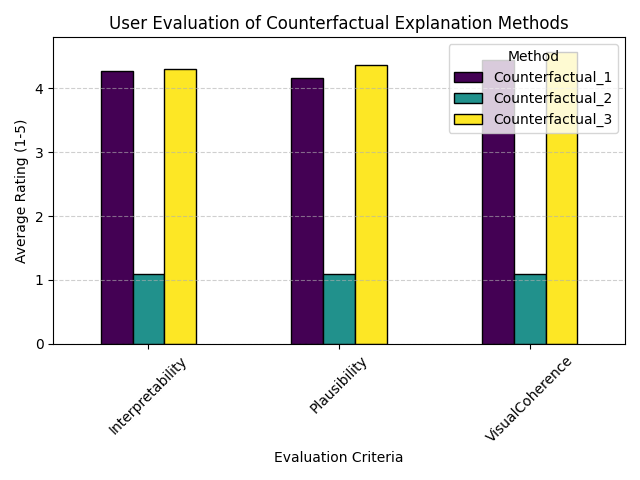
\includegraphics[width=0.7\textwidth]{img/results/bar_plot_user_evaluations.png}
    \caption{User Evaluation of Counterfactual Explanation Methods: Combined Bar Chart}
    \label{fig:barPlotAll}
\end{figure}

\begin{figure}[htbp]
    \centering
    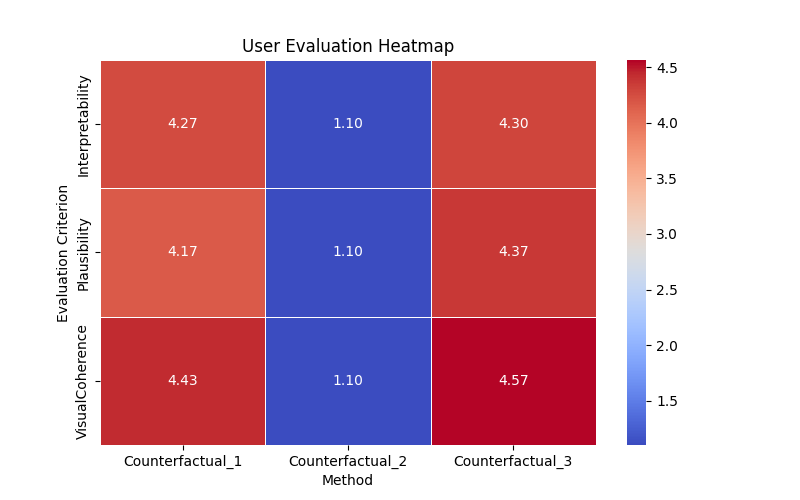
\includegraphics[width=0.7\textwidth]{img/results/heatmap_user_evaluations.png}
    \caption{User Evaluation Heatmap for Three Counterfactual Methods}
    \label{fig:heatmap}
\end{figure}

In addition to these combined views, we generated individual bar charts for each criterion (Figures~\ref{fig:interpretabilityBar}, 
\ref{fig:plausibilityBar}, and \ref{fig:visualCoherenceBar}). Each figure focuses on one metric and plots the average rating 
for each counterfactual method.

\begin{figure}[htbp]
    \centering
    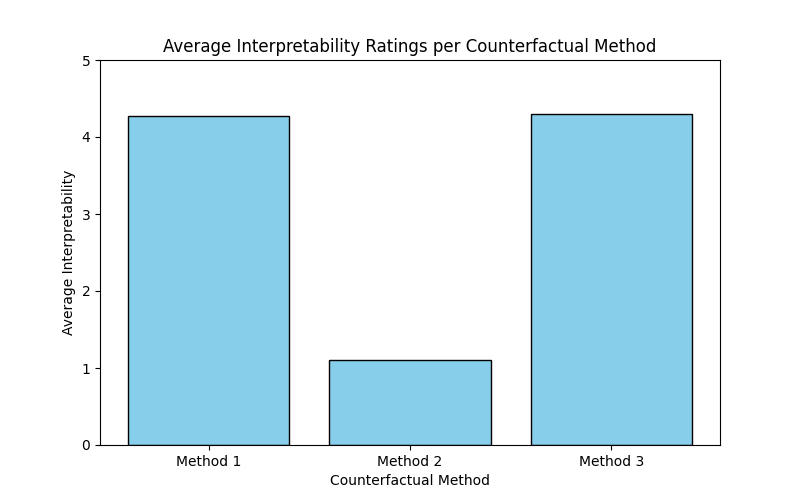
\includegraphics[width=0.55\textwidth]{img/results/Interpretability_ratings.png}
    \caption{Average Interpretability Ratings per Counterfactual Method}
    \label{fig:interpretabilityBar}
\end{figure}

\begin{figure}[htbp]
    \centering
    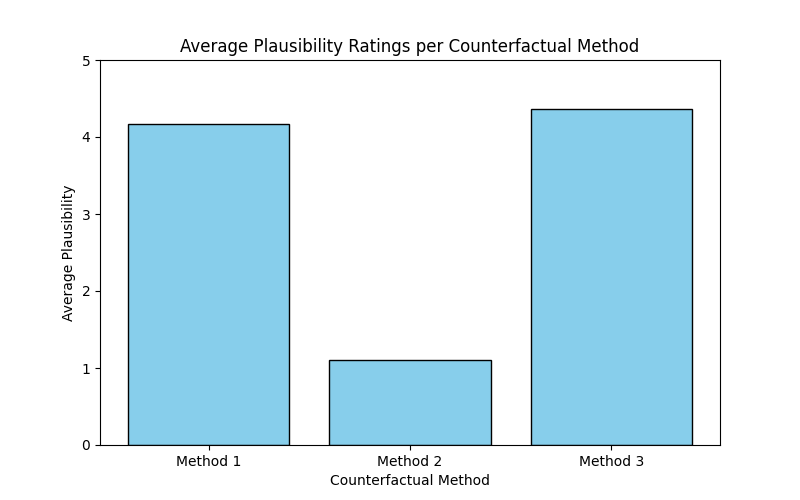
\includegraphics[width=0.55\textwidth]{img/results/Plausibility_ratings.png}
    \caption{Average Plausibility Ratings per Counterfactual Method}
    \label{fig:plausibilityBar}
\end{figure}

\begin{figure}[htbp]
    \centering
    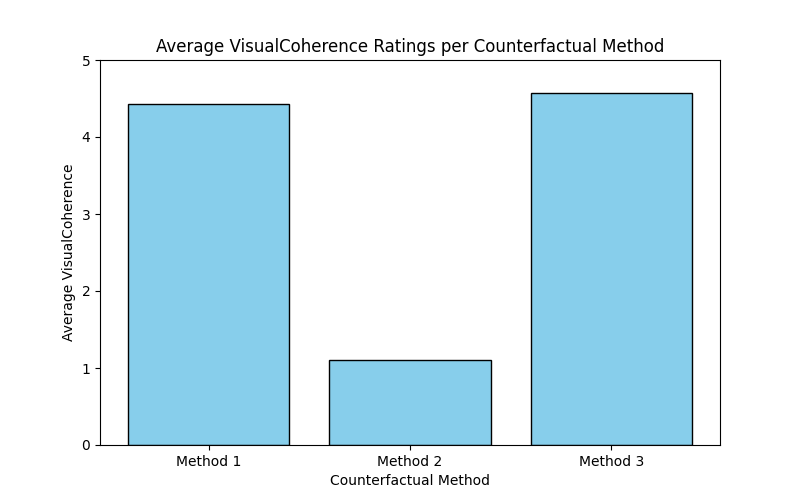
\includegraphics[width=0.55\textwidth]{img/results/VisualCoherence_ratings.png}
    \caption{Average Visual Coherence Ratings per Counterfactual Method}
    \label{fig:visualCoherenceBar}
\end{figure}

Overall, these visualizations indicate that \textbf{Method 3} achieves the highest scores across most metrics, particularly in 
\textit{Visual Coherence} and \textit{Interpretability}, while \textbf{Method 2} often lags behind in \textit{Plausibility} and 
\textit{Visual Coherence}. \textbf{Method 1} offers moderate-to-high performance in most categories but does not surpass Method 3.

\section{Validity}
\label{sec:validity}
Validity is a measure of how often the counterfactual explanation is successfully generated. 
The validity percentage is computed as
\[
\text{Validity (\%)} = \left( \frac{\text{Successful Counterfactuals}}{\text{Total Counterfactuals}} \right) \times 100.
\]

For our methods, a counterfactual is considered valid if it changes the model’s predic-
tion to the desired target class (e.g., from STOP to GO, or from RIGHT to LEFT). 

Table~\ref{tab:validity_results} summarizes the validity results obtained from four different methods:

\begin{table}[htbp]
    \centering
    \caption{Validity of Counterfactual Explanations}
    \label{tab:validity_results}
    \begin{tabular}{lcccc}
        \hline
        \textbf{Method} & \textbf{Total} & \textbf{Successful} & \textbf{Validity (\%)} \\
        & \textbf{Counterfactuals} & \textbf{Counterfactuals} & \\
        \hline
        Grid-Based Masking & 2326 & 2316 & 99.57 \\
        Object Detection & 2326 & 84 & 3.61 \\
        LIME on Images & 2326 & 2044 & 87.88 \\
        LIME on Latent Features & 2326 & 211 & 9.07 \\
        \hline
    \end{tabular}
\end{table}

As seen in Table~\ref{tab:validity_results}, the Grid-Based Masking approach achieved a very high validity of 99.57\%, meaning that nearly all counterfactuals generated by this method were successful. In contrast, the Object Detection method and LIME on Latent Features produced much lower validity values (3.61\% and 9.07\% respectively), indicating that these methods struggled to consistently generate valid counterfactual explanations. LIME on Images yielded a moderately high validity of 87.88\%, suggesting that while it generally succeeds, it does not match the near-perfect performance of Grid-Based Masking.

These findings suggest that the Grid-Based Masking approach is the most robust in generating counterfactual explanations under the conditions tested, while Object Detection and LIME on Latent Features require further refinement to improve their consistency.

\section{Interpretability}
\label{sec:interpretability}
Interpretability refers to the ability to explain or provide the meaning of a system in terms understandable to humans. In our study, 
participants rated each counterfactual on how clear and direct it was in showing \emph{what changed} to alter the AI's decision. 
As shown in Figures~\ref{fig:barPlotAll} and~\ref{fig:interpretabilityBar}, Method 3 obtained the highest average interpretability score.

\section{Plausibility}
\label{sec:plausibility}
Plausibility checks whether the modified (counterfactual) image still looks like a realistic driving scene. If the alterations 
(e.g., removing a pedestrian or adding a turn signal) appear unnatural, the user perceives the explanation as less plausible. 
In Figure~\ref{fig:plausibilityBar}, Method 3 again led in plausibility, while Method 2 often produced blurred or otherwise 
unrealistic modifications, leading to lower user scores.

\section{Visual Coherence}
\label{sec:visualcoherence}
Visual Coherence asks if only the relevant parts of the image are changed while the rest of the scene remains intact. 
This helps isolate the effect of a single element (such as a fallen branch or an oncoming car) on the AI's decision. 
Method 3 excelled here as well, as depicted in Figures~\ref{fig:barPlotAll} and~\ref{fig:visualCoherenceBar}, suggesting 
it can more precisely localize the critical regions in the image.

\subsection{Overall Discussion}
These results suggest that Method 3’s approach to generating counterfactual explanations is most effective at preserving 
scene realism (\textbf{plausibility}) and focusing changes on only the necessary parts (\textbf{visual coherence}) while 
still being easy for users to understand (\textbf{interpretability}). The detailed user feedback and comments support 
these quantitative findings, with many noting that Method 2’s modifications were often “blurred” or “very bad image,” 
explaining its low scores.

Overall, these ratings confirm that focusing on targeted changes and realistic reconstructions significantly enhances 
user perception of counterfactual explanations, an insight that can guide further refinement of deep generative models 
in autonomous driving contexts.